\documentclass[a4paper, itemph]{oblivoir}
\setmainhangulfont{NANUMMYEONGJO.TTF}[BoldFont={NANUMMYEONGJOEXTRABOLD.TTF}]
\usepackage[english]{babel}
\usepackage[utf8x]{inputenc}
\usepackage[T1]{fontenc}
%% Sets page size and margins
\usepackage[a4paper,top=3cm,bottom=2cm,left=3cm,right=3cm,marginparwidth=2cm]{geometry}

\usepackage{indentfirst}

%% Useful packages
\usepackage{amsfonts}
\usepackage{amsmath, mathtools}
\usepackage{graphicx}
\usepackage{subcaption}
\usepackage[colorinlistoftodos]{todonotes}
\usepackage{amssymb}
\usepackage{amsthm}
\usepackage{tikz}

%Extravaganza
\newtheorem{thm}{Theorem}[subsection]
\newtheorem{lem}{Lemma}[subsection]
\newtheorem{cor}{Corollary}[subsection]
\newcommand{\overbar}[1]{\mkern 1.5mu\overline{\mkern-1.5mu#1\mkern-1.5mu}\mkern 1.5mu}
\theoremstyle{definition}
\newtheorem{defn}{Definition}[subsection]
\newtheorem{rem}{Remark}[subsection]

\begin{document}
\title{기초전자회로 및 실험: Lab \#06}
\author{서울대학교 전기$\cdot$정보공학부 2018-12602 이준협}
\maketitle

\section{Preliminaries}
This section serves as a short summary to the model of the drain current that this experiment uses, which was confirmed in lab 5.
\begin{equation}
    I_D = \dfrac{W}{L}C_{ox}\mu_n(V_{GS}-V_{TH}-\dfrac{M}{2}V_{DS})V_{DS}\text{ (Linear region)}
\end{equation}
\begin{equation}
     V_{sat}=\dfrac{V_{GS}-V_{TH}}{M}
\end{equation}
\begin{equation}
    I_{sat} = \dfrac{1}{2M}\dfrac{W}{L}C_{ox}\mu_n(V_{GS}-V_{TH})^2(1+\lambda V_{DS})
\end{equation}
We note that $M$ accounts for the depletion charge near the drain, and in this model it  accounts for velocity saturation also, since $\sqrt{1+\dfrac{2(V_{GS}-V_{TH})}{MLE_{sat}}}+1$ was viewed to be approximately constant. An equation for $M$ in this model can be given as
\[M\approx\dfrac{1+\sqrt{1+\dfrac{2(V_{GS}-V_{TH})}{MLE_{sat}}}}{2}(1+\dfrac{\rho/\sqrt{2\phi_F}}{1+\sqrt{1+\dfrac{V_{DS}}{2\phi_F}}})\approx 1+\dfrac{2.306}{\sqrt{0.6738}+\sqrt{V_{DS}+0.6738}}\]
$\rho$ and $\phi_F$ were measured from the $V_{TH}-V_{SB}$ plot. We also use $\mu_n C_{ox}\dfrac{W}{L}=2600[\mu A/V^2]$, $V_{TH}=1.57[V]$, $\lambda = 1/32[V^{-1}]$ as a rough estimation from the values measured in lab 5. $\mu_n C_{ox}\dfrac{W}{L}\approx 2687[\mu A/V^2]$ when $V_{GS}=1.500[V]$ and $\mu_n C_{ox}\dfrac{W}{L}\approx 2557[\mu A/V^2]$ when $V_{GS}=3.00[V]$, so since our bias point is between the two of them the middle point was taken. Likewise, since $1/\lambda\approx 30.95[V]$ when $V_{GS}=1.500[V]$ and $1/\lambda\approx 33.45[V]$ when $V_{GS}=3.00[V]$, the middle point was taken.

We calculate $g_m$, $r_o$ and $A_v$ as $g_m=\dfrac{\partial I_{sat}}{V_{GS}}=\dfrac{1}{M}\dfrac{W}{L}C_{ox}\mu_n(V_{GS}-V_{TH})(1+\lambda V_{DS})\\=\sqrt{\dfrac{2}{M}\dfrac{W}{L}C_{ox}\mu_n(1+\lambda V_{DS})I_{sat}}$, $r_o=\dfrac{1/\lambda+V_{DS}}{I_{sat}}$, and $A_v=-g_m(r_o||R_D)$. Note that $V_{DS}=V_{out}$, $I_{sat}=\dfrac{V_{DD}-V_{out}}{R_D}$, so all we have to measure is $R_D$, $V_{in}$, and $V_{out}$ at the bias point.

\section{Inverter Voltage Transfer Curve}

\begin{figure}[htb]
    \centering
    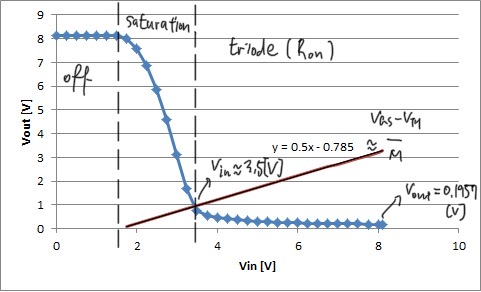
\includegraphics[width=0.5\linewidth]{vtc.JPG}
    \caption{The VTC of the inverter with a resistor $R_D=3.03[k\Omega]$ as the pullup device.}
\end{figure}

$M\approx 1.6$ when $V_{DS}=V_{out}=8.12[V]=V_{DD}$, and $M\approx 2.4$ when $V_{DS}=V_{out}=0$, so we use $M\approx 2$ and therefore $V_{D,sat}=\dfrac{V_{GS}-V_{TH}}{M}\approx \dfrac{V_{in}-1.57}{2}$ as an approximation to the saturation voltage. That is, when $V_{out}$ is above the red line in figure 1, the NMOS is in saturation.

Therefore, we see that when the NMOS is below the threshold voltage of $1.57[V]$, the NMOS is off and therefore the voltage is pulled up to $V_{DD}$. Then the NMOS is turned on and is in saturation mode, therefore $V_{out}=V_{DD}-I_DR_D$ is quadratic. Finally, the NMOS reaches the triode region above $V_{out}\approx 3.50[V]$ and becomes a resistor with $R_{on}=\dfrac{1}{\mu_n C_{ox}\dfrac{W}{L}(V_{in}-V_{TH})}$. This expression for the on resistance can be confirmed by calculating the output voltage at $V_{in}=V_{DD}=8.12[V]$ by viewing the inverter as a voltage divider. $R_{on}=\dfrac{1}{2600\cdot (8.12-1.57)}=5.872\times 10^{-5}[M\Omega ]=58.72[\Omega]$, so $V_{out}=8.12\times \dfrac{58.72}{58.72+3030}=0.154[V]$. The measured value is $0.1957[V]$, so the error is $(\dfrac{1957}{1540}-1)\times 100=27.08\%$. This is due to the decreased mobility due to the increase in gate voltage. When we calculate $\mu_n C_{ox}\dfrac{W}{L}$ from $R_{on}=\dfrac{3030\times 0.1957}{8.12-0.1957}=74.83[\Omega]=\dfrac{1}{\mu_n C_{ox}\dfrac{W}{L}\cdot (8.12-1.57)}$, we get $\mu_n C_{ox}\dfrac{W}{L}=2034[\mu A/V^2]<2600[\mu A/V^2]$. Since the mobility parameter was measured to be keep decreasing when the gate voltage increases, this result can be explained with theory, as the recalculated mobility parameter is of the same order.
\section{Small Signal Gains}
\begin{figure}[htb]
    \centering
    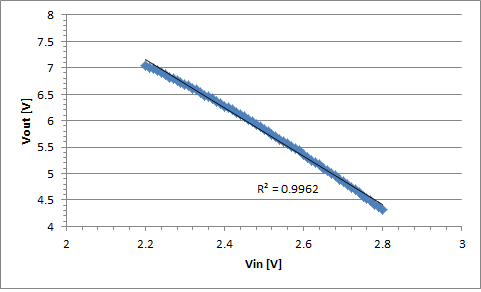
\includegraphics[width=0.4\linewidth]{3030_gain.png}
    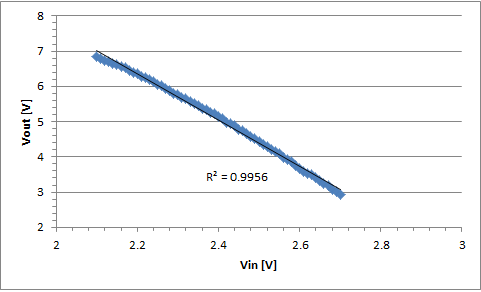
\includegraphics[width=0.4\linewidth]{5050_gain.png}
    \caption{$V_{in}$ incremented by 0.01[V]. Left: $R_D=3.03[k\Omega]$, bias point $V_{in}=2.50[V]$. Right: $R_D=5.05[k\Omega]$, bias point $V_{in}=2.40[V]$.}
\end{figure}

The bias points were chosen to be approximately in the middle of the saturation region of the VTC. When the output voltages were measured each time the input voltage was raised by $0.01[V]$, the data fitted the linear model well, with $R^2=0.9962/0.9956$ for $R_D=3.03/5.05[k\Omega]$.

The voltage swing of the input voltage was from $2.20[V]$ to $2.80[V]$ when $R_D=3.03[k\Omega]$, and when $R_D=5.05[k\Omega]$ the voltage swing is from $2.10[V]$ to $2.70[V]$. The output voltage swing was from $7.05[V]$ to $4.31[V]$/$6.85[V]$ to $2.94[V]$. Therefore, $A_v=\dfrac{4.31-7.05}{2.80-2.20}=-4.57[V/V]$ when $R_D=3.03[k\Omega]$, and $A_v=\dfrac{2.94-6.85}{2.70-2.10}=-6.52[V/V]$ when $R_D=5.05[k\Omega]$.
\begin{table}[htb]
    \centering
    \begin{tabular}{c|c|c|c|c|c}
        $R_D[k\Omega]$ & $V_{out}[V]$ & $I_{sat}[mA]$ & $g_m[mA/V]$ & $r_o[k\Omega]$ & $A_v[V/V]$\\
        \hline
        3.03 & 5.84 & 752 & 1.53 & 50.3 & -4.36\\
        \hline
        5.05 & 5.14 & 590 & 1.34 & 62.9 & -6.26
    \end{tabular}
    \caption{A summary of the small-signal gains calculated from using the equations in section 1. $M=1+\dfrac{2.306}{\sqrt{0.6738}+\sqrt{V_{DS}+0.6738}}$, $\mu_n C_{ox}\dfrac{W}{L}=2600[\mu A/V^2]$, $1/\lambda = 32[V]$, $g_m=\sqrt{\dfrac{2}{M}\dfrac{W}{L}C_{ox}\mu_n(1+\lambda V_{DS})I_{sat}}$, $r_o=\dfrac{1/\lambda+V_{DS}}{I_{sat}}$, and $A_v=-g_m(r_o||R_D)$}
\end{table}

The error between the calculated values of $A_v$ and the measured values are $\left|\dfrac{-4.56+4.36}{-4.36}\right|\times 100=4.82\%$ for $R_D=3.03[k\Omega]$, and $\left|\dfrac{-6.52+6.26}{-6.26}\right|\times 100=4.15\%$ for $R_D=5.05[k\Omega]$. It can be observed that the measured values fits well with theory, with approximate errors below $5\%$. This error is from the fact that the VTC is not entirely quadratic, since $M$ and $\mu_n C_{ox}\dfrac{W}{L}$ are values that depend on $V_{DS}$ and $V_{GS}$. Especially, since the body effect is significant, we expect the variation of $M$ to affect the $\sqrt{1/M}$ term in $g_m$. Also, the value of $1/\lambda$ increases when $V_{DS}$ increases, so $r_o$ increases and therefore $R_D||r_o$ increases. That may be the reason why the measured gain is larger than the expected gain.
\begin{thebibliography}{}

\bibitem{1} S. M. Sze and K. K. Ng, \textit{Physics of Semiconductor Devices}, 4th ed. Hoboken, NJ: Wiley, 2015.

\end{thebibliography}

\end{document}
